\section{Résultats}

\paragraph{Mesures initiales} Les dimensions des échantillons de titane, laiton et acier doux étudiés ainsi que leur masse et masse volumique \(\rho = \frac{m}{L \ell e}\) sont reportés dans le \autoref{tab:dimensions}.

\begin{table}[h]
    \centering
    \begin{tabulary}{0.7\linewidth}{c|c c c c c}
        \toprule
        Échantillon & \(e\) [\si{\milli\meter}] & \(\ell\) [\si{\milli\meter}] & \(L\) [\si{\milli\meter}] & \(m\) [\si{\gram}] & \(\rho\) [\si{\gram\per\cubic\centi\meter}] \\
        \midrule
        Titane & \(2.10 \pm 0.02\) & \(5.03 \pm 0.02\) & \(59.38 \pm 0.03\) & \(2.6556 \pm 0.0005\) & \(4.23 \pm 0.04\) \\
        Laiton & \(2.01 \pm 0.02\) & \(5.95 \pm 0.02\) & \(60.00 \pm 0.03\) & \(5.9803 \pm 0.0005\) & \(8.33 \pm 0.08\) \\
        Acier doux & \(1.53 \pm 0.02\) & \(4.09 \pm 0.02\) & \(58.84 \pm 0.03\) & \(2.7658 \pm 0.0005\) & \(7.5 \pm 0.1\) \\
        \bottomrule
    \end{tabulary}
    \caption{Dimensions, masse et masse volumique de chaque échantillon}
    \label{tab:dimensions}
\end{table}

\paragraph{Module de Young} Pour chacun des échantillons, le module de Young \(E\) à température ambiante de \(T = (295 \pm 1)\) \si{\kelvin} a été obtenu avec l'\autoref{eq:young_programme}. La fréquence fondamentale de vibration, ainsi que le module de Young pour chacun des échantillons sont recensées dans le \autoref{tab:young_amortissement}.

\paragraph{Capacité d'amortissement} En plus du module de Young, le programme calcule aussi, en utilisant l'\autoref{eq:q1_programme}, la capacité d'amortissement \(Q^{-1}\). Cette mesure est réalisé plusieurs fois sur le même échantillon. Le \autoref{tab:young_amortissement} reporte la valeur moyenne et leur déviation pour chaque échantillon.

\begin{table}[h]
    \centering
    \begin{tabulary}{\linewidth}{c|c c c C C}
        \toprule
        Échantillon & \(f\) [\si{\per\second}] & \(E\) [\si{\giga\pascal}] & \(E_\textrm{ref}\) [\si{\giga\pascal}] \cite{notice-d1} & Erreur relative sur \(E\) & \(Q^{-1}\) \\
        \midrule
        Titane & \(3094 \pm 1\) & \(108 \pm 3\) & \(115.7\) & 6\% & \(\left(7.20 \pm 0.02\right) \cdot 10^{-5}\) \\
        Laiton & \(2000 \pm 1\) & \(101 \pm 3\) & \(100.6\) & 1\% & \(\left(5.32 \pm 0.05\right) \cdot 10^{-5}\) \\
        Acier doux & \(2228 \pm 1\) & \(180 \pm 7\) & \(211.9\) & 14\% & \(\left(2.61 \pm 0.04\right) \cdot 10^{-4}\) \\
        \bottomrule
    \end{tabulary}    
    \caption{Fréquence fondamentale, module de Young et capacité d'amortissement obtenues à température ambiante \(T = (295 \pm 1)\) pour chacun des échantillons}
    \label{tab:young_amortissement}
\end{table}

\paragraph{Module de Young et température} Afin d'observer les effets de la température sur un échantillon d'acier doux, le module de Young a été déterminé pour des températures entre \mbox{\(T = (299 \pm 1)\) \si{\kelvin}} et \mbox{\(T = (525 \pm 1)\) \si{\kelvin}}. Les résultats sont reportés dans la \autoref{fig:module_young_temp}.

\begin{figure}[h]
    \centering
    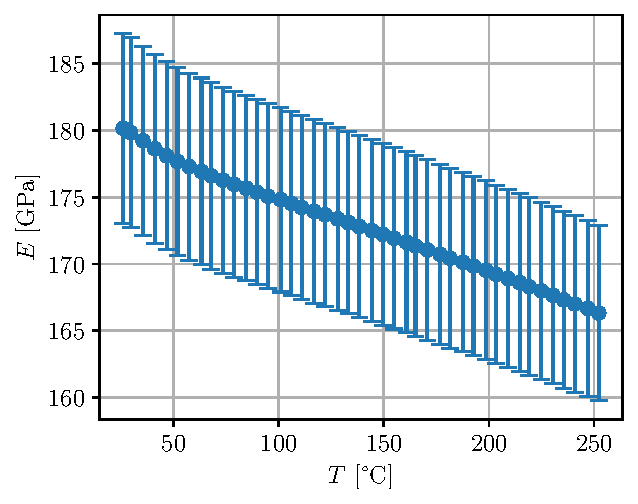
\includegraphics[width=0.6\linewidth]{figures/acier_doux_module_young_temp.pdf}
    \caption{Module de Young d'un échantillon d'acier doux en fonction de la température}
    \label{fig:module_young_temp}
\end{figure}

\paragraph{Frottement intérieur et température} Afin de déterminer plusieurs caractéristiques supplémentaires de l'acier doux en relaxation inélastique des mesures du frottement intérieur en fonction de la température $Q^{-1}(T)$ ont été effectuées. Le pic prédit par l'\autoref{eq:Q_inv_T} à $T_P$ a été observé et étudié, il est visible dans les \autoref{fig:acier_doux_temp_unadjusted} et \autoref{fig:acier_doux_temp_adjusted}.

En raison d'une accumulation d'erreurs sur la durée de la mesure, une régression quadratique a été réalisée afin de corriger les valeurs obtenues. La sortie non-traitée du programme pour $Q^{-1}$ ainsi que la régression sont visibles en \autoref{fig:acier_doux_temp_unadjusted}. Afin d'obtenir un pic plat sans cette erreur la valeur de la fonction $y$ obtenue par la régression a été soustraite à tous les points et le résultat est affiché en \autoref{fig:acier_doux_temp_adjusted}.

\begin{figure}[h]
    \centering
    \begin{subfigure}{0.6\linewidth}
        \centering
        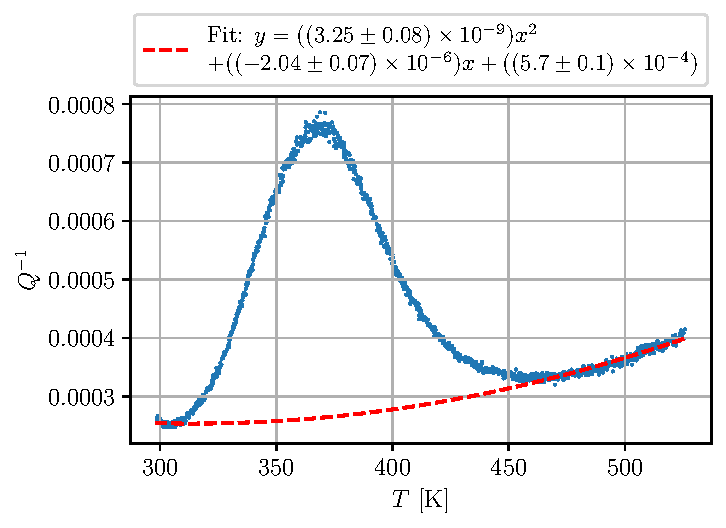
\includegraphics[width=\linewidth]{figures/acier_doux_q_1_temp_unadjusted.pdf}
        \caption{}
        \label{fig:acier_doux_temp_unadjusted}
    \end{subfigure}
    \begin{subfigure}{0.6\linewidth}
        \centering
        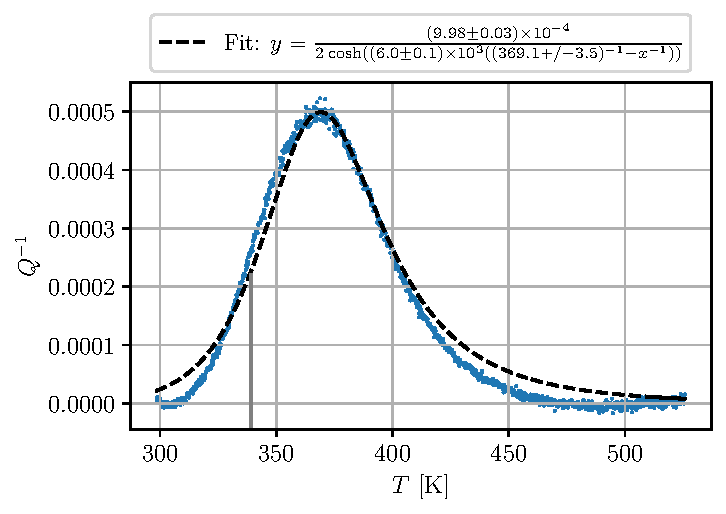
\includegraphics[width=\linewidth]{figures/acier_doux_q_1_temp_adjusted.pdf}
        \caption{}
        \label{fig:acier_doux_temp_adjusted}
    \end{subfigure}
    \caption{Frottement interieur \(Q^{-1}\) pour un échantillon d'acier doux (a) avec l'erreur quadratique (b) sans l'erreur quadratique}
\end{figure}

Le pic obtenu permet de déduire plusieurs informations. Tout d'abord il a pu être extrait du graphique $\Delta / 2 = (5.2 \pm 0.2) \times 10^{-4}$ . Ensuite les valeurs de $T_P$, $T_1$ et $T_2$ telles que définies pour les \autoref{eq:Q_inv_T} et \autoref{eq:H_mi_hauteur} ont pu être estimées. Pour $T_P$ toutes les valeurs proches de moins $10^{-5}$ du point maximal selon $Q^{-1}$ ont été sélectionnées. La moyenne de cet échantillon ainsi que l'écart entre les deux éléments les plus éloignés a donné la valeur et l'erreur pour $T_P = (369 \pm 3)$ \si{\kelvin}. Pour $T_1$ et $T_2$ tous les points pour lesquels la barre de mi-hauteur $\Delta / 4$ était franchie en ce point étaient sélectionnés, et triés selon leur proximité entre $T_1$ et $T_2$. Pareillement les valeurs moyennes et les écarts entre les extrêmes ont donnés: $T1 = (339.7 \pm 0.7)$ \si{\kelvin} et \mbox{$T2 = (400 \pm 1)$ \si{\kelvin}}.

A l'aide de ces valeurs et de l'\autoref{eq:H_mi_hauteur} la valeur de l'énergie de diffusion obtenue est: $H = (8.2 \pm 0.2)\times 10^{-20}$.

Les données corrigées en \autoref{fig:acier_doux_temp_adjusted} correspondant à l'\autoref{eq:Q_inv_T} une régression a été appliquée à ces valeurs avec les valeurs connues de $H$, $k_b$ et $T_P$. Une valeur pour l'intensité de relaxation de \(\Delta = (9.98 \pm 0.03) \times 10^{-4}\) est alors obtenue. La valeur de $\Delta$ conservée est celle obtenue par la régression plus précise que celle obtenue par analyse du graphique. 


\paragraph{Concentration de carbone interstitiel}

$J_u = 1/E$, $k_b$, $T_P$ et $\Delta$ sont connus pour l'acier doux grâce aux études précédentes. Sachant que les défauts interstitiels sont du carbone il est donné que $\Delta\lambda = 0.62$ et $v_0 = 3.05 \times 10^{-30}$ \si{\cubic\meter} tels que définis pour l'\autoref{eq:delta_defauts}. Il est possible de calculer la concentration en carbone interstitiels dans l'acier doux étudié par l'\autoref{eq:c_0}: $c_0 = (1.08 \pm 0.04)\times 10^{-4}$.